\chapter{Artificial neural networks}

Sztuczne sieci neuronowe mają obecnie bardzo mocno ugruntowaną pozycję szczególnie w dziedzinie problemów związanych z analizą i przetwarzaniem obrazów. Pomimo, iż nie jest to nowy pomysł, dopiero ostatni wzrost w wydajności komputerów pozwolił na ich praktyczne zastosowanie. Z matematycznego punktu widzenia są to sparametryzowane nieliniowe funkcje o pewnej ustalonej strukturze. Składają się z prostych elementów zwanych neuronami, a one natomiast są pogrupowane w warstwy. Połączenia między warstwami definiują przepływ danych. 'Nauka' sieci neuronowych polega na optymalizacji pewnej funkcji straty, czyli wyznaczeniu takich parametrów, żeby osiągnąć minimalny koszt. Do tego celu często korzysta się z metod opartych na SGD, a przy wybranej strukturze można w efektywny sposób zastosować algorytm propagacji wstecznej. W dalszej części pracy będę używał prostszej nazwy (neural nets). Przykładowa architektura sieci neuronowych jest zaprezentowana na wykresie ???.

\section{Autoencoders}

Jest to jeden z rodzajów sieci neuronowych, służący do znajdowania wydajnej reprezentacji danych, co jest przykładem nauki bez nadzoru. W autoencoder'ach mozna wyróżnić dwie części: encoder i decoder. Zadaniem encodera jest wyprodukowanie reprezentacji, natomiast decoder służy do odtworzenia z niej oryginalnej postaci. Zależy nam na tym, żeby wyjście było w jakimś sensie jak najbardziej podobne do wejścia. W przypadku obrazów jako funkcja straty często stosowane jest MSE. Przykładowy schemat na wykresie \ref{fig:autoenc}.

\begin{figure}
    \centering
    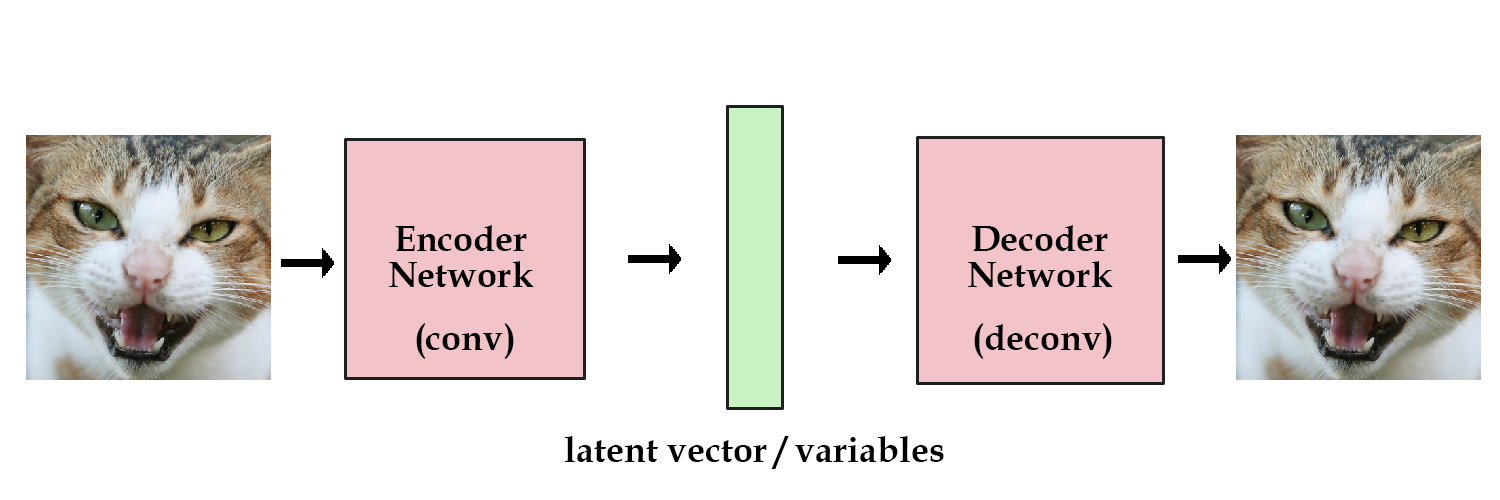
\includegraphics[width=1\textwidth]{images/autoenc}
    \caption{Architecture of autoencoder}
    \label{fig:autoenc}
\end{figure}

\section{VAE}

Variational autoencoders rezszerzają założenia o wprowadzenie modelowania rozkładu prawdopodobieństwa dla reprezentacji ukrytej. 

\section{Convolution VAE}

Jest to rozszerzenie poprzedniego modelu, w którym dodatkowo stosujemy warstwy splotowe. Szczególnie w przypadku obrazów pozwala to na zwiększenie rozmiaru danych wejściowych przez zmniejszenie ilości parametrów w stosunku do warstw fully-connected oraz wykryciu na wstępie jakiś prostych cech, przez co w reprezentacji mogą znajdowac się bardziej abstrakcyjne rzeczy. 

\section{Deep feature consistent variational auto-encoder}

Ta wersja zakłada użycie innej funkcji kosztu. MSE z samej definicji przyczynia się do uśredniania wartości pikseli przez co wyjściowy obraz nie jest wyraźny. W tym przypadku będziemy korzystać z zewnetrznej sieci splotowej wyuczonej do klasyfikacji obrazów. Będziemy teraz myśleć, że dwa obrazy są podobne, jeśli maja podobne wartości aktywacji w tej sieci. Takie podejście powinno nam dać ostrzejsze wyjście.
